\documentclass[hidelinks, 12pt]{article}
\usepackage[italian]{babel}
\usepackage{natbib}
\usepackage{url}
\usepackage[utf8x]{inputenc}
\usepackage{amsmath}
\usepackage{graphicx}
\graphicspath{{images/}}
\usepackage{parskip}
\usepackage{fancyhdr}
\usepackage{vmargin}
\usepackage{float}
\usepackage{hyperref}
\usepackage{subfig}
\setmarginsrb{3 cm}{2.5 cm}{3 cm}{2.5 cm}{1 cm}{1.5 cm}{1 cm}{1.5 cm}

\title{Amazon Reviews Sentiment Analysis}				% Title
\author{Basso Matteo \\ Ferri Marco}								% Author
\date{Luglio 2019}				% Date

\makeatletter
\let\thetitle\@title
\let\theauthor\@author
\let\thedate\@date
\makeatother

\pagestyle{fancy}
\fancyhf{}
\rhead{Basso M., Ferri M.}
\lhead{\thetitle}
\cfoot{\thepage}

\begin{document}
	
%%%%%%%%%%%%%%%%%%%%%%%%%%%%%%%%%%%%%%%%%%%%%%%%%%%%%%%%%%%%%%%%%%%%%%%%%%%%%%%%%%%%%%%%%

\begin{titlepage}
	\centering
	\vspace*{0.5 cm}
	
\includegraphics[scale = 0.75]{images/LogoBicocca.pdf}\\[1.0 cm]	% University Logo
	\textsc{\LARGE Università degli studi di}\\[0.2 cm]
	\textsc{\LARGE Milano-Bicocca}\\[2.0 cm]	% University Name
	\textsc{\Large F1801Q127}\\[0.5 cm]				% Course Code
	\textsc{\large Data Analytics}				% Course Name
	\rule{\linewidth}{0.2 mm} \\[0.4 cm]
	{ \huge \bfseries \thetitle}\\
	\rule{\linewidth}{0.2 mm} \\[1.5 cm]
	
	\begin{minipage}{0.4\textwidth}
		\begin{flushleft} \large
			\emph{Studenti:}\\
			\theauthor
		\end{flushleft}
	\end{minipage}~
	\begin{minipage}{0.4\textwidth}
		\begin{flushright} \large
			\emph{Matricole:} \\
			807628 \\ 807130
		\end{flushright}
	\end{minipage}\\[2 cm]
	
	{\large \thedate}\\[2 cm]
	
	\vfill
	
\end{titlepage}

%%%%%%%%%%%%%%%%%%%%%%%%%%%%%%%%%%%%%%%%%%%%%%%%%%%%%%%%%%%%%%%%%%%%%%%%%%%%%%%%%%%%%%%%%


\null\vspace{\stretch{1}}
\section*{\centering Abstract}

Lorem ipsum dolor sit amet.

\vspace{\stretch{2}} \null

\clearpage


%%%%%%%%%%%%%%%%%%%%%%%%%%%%%%%%%%%%%%%%%%%%%%%%%%%%%%%%%%%%%%%%%%%%%%%%%%%%%%%%%%%%%%%%%

\tableofcontents
\clearpage
\listoffigures
\listoftables
\pagebreak

%%%%%%%%%%%%%%%%%%%%%%%%%%%%%%%%%%%%%%%%%%%%%%%%%%%%%%%%%%%%%%%%%%%%%%%%%%%%%%%%%%%%%%%%%



\section{Introduzione}


Lo studio ha lo scopo di condurre diversi tipi di analisi sulle recensioni del noto portale e-commerce Amazon \cite{site:amazon}. In questa sezione viene presentata una breve introduzione al problema, il dataset utilizzato e gli strumenti che sono stati impiegati per portare a termini gli obiettivi prefissati.



\subsection{Dominio di riferimento}

Sempre maggiore è il numero di siti web che fanno delle recensioni il proprio principale business. Si pensi ai portali dedicati alla recensione di località turistiche, film o ristoranti. Allo stesso modo, anche Amazon basa sulle recensioni parte della propria fidelizzazione clienti.

Trattandosi di dati testuali prodotti dagli utenti per valutare i prodotti acquistati, le recensioni esprimono attraverso il linguaggio naturale le impressioni dell'autore, le quali possono assumere un carattere di natura positiva o negativa. In questo contesto è inoltre pratica comune associare al proprio pensiero un punteggio che esprima una valutazione del prodotto su una scala numerica. Se questa informazione è fondamentale per i clienti della piattaforma, poiché permette di capire a colpo d'occhio quale possa essere la qualità dell'articolo che si sta considerando di acquistare, è anche vero che tale punteggio possa rappresentare un aiuto importante per riassumere in forma strutturata (e pertanto più facilmente comprensibile da un computer) l'opinione dell'autore riguardo un certo argomento. Pertanto, analizzare congiuntamente il testo di una recensione ed il punteggio ad essa associato è fondamentale per determinare una correlazione fra il linguaggio naturale e l'opinione dell'utente nei confronti del prodotto, anche detta \textbf{sentiment}. Inoltre, l'elaborazione del testo può considerare il piano morfologico del linguaggio per derivare l'opinione espressa riguardo le diverse caratteristiche del prodotto, dette \textbf{aspect}, espresse della recensione. Ciò è particolarmente utile per migliorare la qualità dei propri prodotti e ottenere quindi un vantaggio sul piano commerciale.

Infine, l'analisi delle recensioni può essere utile anche per ottenere un'approssimativa profilazione di un utente; questa può rivelarsi particolarmente rilevante dal punto di vista del marketing, ad esempio per dare suggerimenti ad altri utenti che dimostrano di avere le medesime preferenze del primo. Allo stesso modo, può essere costruito anche un sistema di suggerimenti basato su prodotti simili o solitamente venduti insieme. Tali tecniche vengono dette di \textbf{collaborative filtering}.

Il seguente elaborato si pone l'obiettivo di sperimentare con i concetti appena presentati per determinare quanto sia possibile ottenere attraverso l'analisi delle recensioni di un portale e-commerce come Amazon.



\subsection{Dataset}

Il dataset utilizzato per effettuare le analisi è fornito ufficialmente da Amazon e contiene recensioni redatte fra il 1996 e il 2014, per diverse categorie di prodotti \cite{site:amazon-reviews-original-dataset}. Poiché contenente un gran numero di recensioni che coinvolgono altrettanti utenti e prodotti, talvolta poco partecipativi all'interno del portale e-commerce, si è scelto di utilizzare ai fini del progetto una versione rielaborata del suddetto dataset, reperibile qui: \url{http://jmcauley.ucsd.edu/data/amazon}. Julian McAuley \cite{site:julianmcauley}, professore dell'Università di San Diego, ha estrapolato dal dataset originale solamente i record delle recensioni riguardanti prodotti e utenti con almeno cinque recensioni ciascuno; ciò viene definito in teoria dei grafi con il termine \textbf{k-core}, cioè un sottografo in cui tutti i nodi hanno un grado almeno pari a \texttt{k}.

\nocite{site:amazon-reviews-5-core-dataset}



\subsection{Strumenti}

Per effettuare le analisi mostrate in questo elaborato si è utilizzato prevalentemente il linguaggio di programmazione open source Python, attraverso l'utilizzo di Google Colab \cite{site:google-colab} per la creazione di Jupyter Notebook interattivi. Le specifiche librerie di volta in volta utilizzate saranno presentate contestualmente alle singole analisi qualora lo si ritenesse necessario ai fini di una migliore comprensione del problema.

Per l'analisi della rete di prodotti e utenti ricavata dal dataset si è utilizzato il software Cytoscape \cite{site:cytoscape}, dedicato appositamente all'integrazione e visualizzazione di grafi anche molto complessi. Nell'ultima parte del documento verrà infine presentata una demo Web-based per testare con mano le potenzialità dei concetti studiati.



\clearpage



\section{Basic Analysis}


Il dataset è stato reperito in formato JSON e successivamente letto attraverso Python per la memorizzazione in una struttura adatta ad essere elaborata efficientemente dal linguaggio. A tal fine si è scelto di utilizzare la liberia \texttt{pandas} \cite{site:pandas}, dedicata all'analisi di dati anche molto voluminosi. É interessante notare come la lettura del dataset, ed in particolare la conversione di quest'ultimo dal formato JSON, sia stata una delle operazioni computativamente più \textit{time-consuming} fra tutte quelle effettuate, a dimostrazione del fatto che \texttt{pandas} sia successivamente in grado di elaborare molto velocemente le informazioni memorizzate all'interno dei cosiddetti \texttt{DataFrame}.



\subsection{Schema}

Il dataset può essere descritto molto velocemente, poiché rappresentabile attraverso una singola struttura tabellare composta dai campi illustrati in tabella \ref{tab:df-schema}.

\begin{table}[H]
	\caption{Schema originale del dataset}\label{tab:df-schema}
	\centering
	\begin{tabular}{|l|l|l|}
		\hline
		Campo & Descrizione \\
		\hline
		reviewerID & ID utente \\
		reviewerName & Nome utente \\
		asin & ID prodotto \\
		reviewText & Testo della recensione \\
		summary & Titolo della recensione \\
		helpful & Utilità della recensione \\
		overall & Punteggio \\
		reviewTime & Timestamp in formato string \\
		unixReviewTime & Timestamp in formato unix \\
		\hline
	\end{tabular}
\end{table}

Ogni record è la rappresentazione di una singola recensione, svolta da parte di un utente per un certo prodotto nella data indicata. Mentre per quanto riguarda l'utente si è in possesso sia dell'ID che del nome (che non verrà utilizzato), il prodotto è rappresentato nel dataset solamente attraverso un ID (\texttt{asin}); ulteriori dettagli sul prodotto possono essere ricavati contattando il creatore del dataset attraverso un'apposita richiesta, che non è stata effettuata poiché tali informazioni si sono rivelate ininfluenti ai fini del progetto in esame.

Per quanto riguarda i campi relativi alla recensione, è possibile visualizzare sia il titolo che il testo del corpo, oltre al punteggio espresso su una scala numerica da 1 a 5. Poiché ciò rappresenta il sentiment associato alla recensione, questo attributo costituirà anche la variabile target per l'analisi e l'addestramento dei modelli di machine learning.

Il campo \texttt{helpful} non è definito su un preciso dominio e pertanto si è scelto di ignorarlo. Per il timestamp è stato computato un campo \texttt{date} di tipo \textit{datetime} e per semplificare il concetto associato ad ogni campo si è scelto di rinominarli. Al termine della trasformazione, il dataset risultante è il seguente:

\begin{table}[H]
	\caption{Schema modificato del dataset}\label{tab:df-schema}
	\centering
	\begin{tabular}{|l|l|l|}
		\hline
		Campo & Descrizione \\
		\hline
		userID & ID utente \\
		productID & ID prodotto \\
		text & Testo della recensione \\
		summary & Titolo della recensione \\
		rating & Punteggio \\
		date & Timestamp in formato datetime \\
		\hline
	\end{tabular}
\end{table}



\subsection{Dimensioni}

Dalla fonte citata nell'introduzione, da cui è stato reperito il dataset, è possibile notare che siano presenti varie possibilità di download. Diverse categorie di prodotti sono state testate durante l'intero sviluppo dello studio, ma ai fini di redigere questo elaborato verrà considerato il dataset 5-core chiamato \textit{Clothing, Shoes and Jewelry}, contenente recensioni relative al mercato dei vestiti, delle scarpe e dei gioielli.

Questo contiene un totale di \textbf{278.677 recensioni}, divise fra \textbf{39.387 utenti} e \textbf{23.033 prodotti}. Ciò significa una media di circa 7 recensioni ad utente e 12 recensioni per prodotto. Nel capitolo \ref{sec:network-anal} verrà mostrata se tale media è anche effettivamente rappresentativa del dataset oppure diversi prodotti ed utenti presentano un numero di recensioni sbilanciato.



\subsection{Distribuzione di \texttt{rating}}

In figura \ref{fig:rating-distr-orig} è possibile osservare la distribuzione del campo \texttt{rating}, che costituisce l'elemento fondamentale su cui costruire un modello supervisionato di sentiment analysis. Come è possibile osservare, questa variabile è fortemente sbilanciata sui valori 4 e 5, motivo che a fronte di alcune considerazioni future porterà il problema ad essere prima binarizzato e successivamente downsampled per ridurre il gap fra la classe positiva e quella negativa.

\begin{figure}[H]
	\centering
	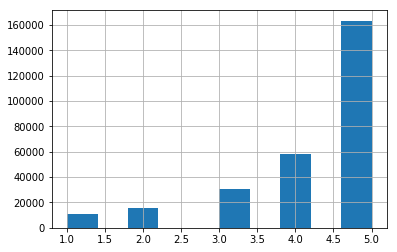
\includegraphics[scale=0.7]{images/02_01_rating_distr.png}
	\caption[Distribuzione del campo \texttt{rating}]{Distribuzione del campo \texttt{rating}}
	\label{fig:rating-distr-orig}
\end{figure}



\subsection{Analisi temporale business-oriented}

Si era già accennato che la fonte fornisca recensioni per più di dieci anni di vendite. Più precisamente, il dataset qui considerato considera recensioni fra il marzo 2003 e giugno 2014 secondo la distribuzione indicata in figura \ref{fig:date-distr}. Pur essendo la maggior parte delle recensioni concentrata negli ultimi 3 anni, qualsiasi sia il filtro temporale applicato non c'è differenza nella distribuzione della variabile target.

\begin{figure}[H]
	\centering
	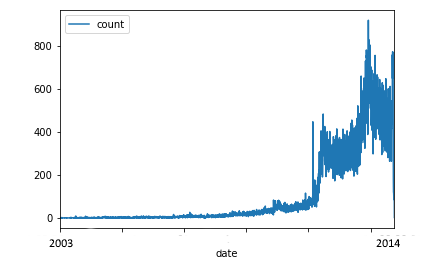
\includegraphics[scale=0.7]{images/02_02_date_distr.png}
	\caption[Distribuzione delle recensioni per data]{Distribuzione delle recensioni per data}
	\label{fig:date-distr}
\end{figure}

\clearpage

Considerato il dominio in esame, potrebbe essere molto utile nell'ottica di prendere decisioni di business per i produttori analizzare come le recensioni si distribuiscono anche in un anno relativamente ai mesi e i giorni della settimana, per evidenziare eventuali periodi di maggiore attività su Amazon. A tal proposito sono pertanto stati prodotti i grafici in figura \ref{fig:month-distr} e \ref{fig:day-distr}.

\begin{figure}[H]
	\centering
	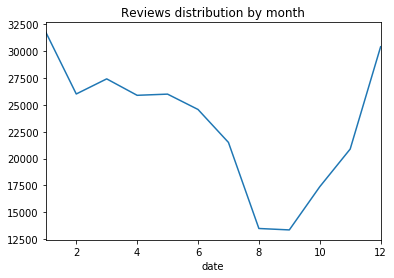
\includegraphics[scale=0.7]{images/02_03_month_distr.png}
	\caption[Distribuzione delle recensioni per mese]{Distribuzione delle recensioni per mese}
	\label{fig:month-distr}
\end{figure}

\begin{figure}[H]
	\centering
	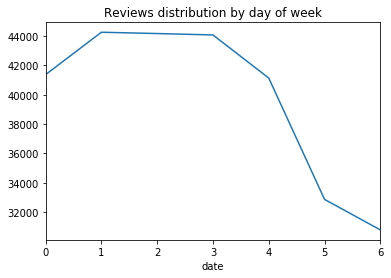
\includegraphics[scale=0.7]{images/02_04_day_distr.png}
	\caption[Distribuzione delle recensioni per giorno della settimana]{Distribuzione delle recensioni per giorno della settimana}
	\label{fig:day-distr}
\end{figure}

Osservando la distribuzione per mese, è possibile notare come la maggiore concentrazione di recensioni si riscontri nel periodo compreso fra il black friday (Novembre) e tutte le vacanze natalizie, probabilmente proprio per via degli sconti e della necessità di comprare regali ai propri conoscenti. É durante questi mesi e quelli immediatamente precedenti che i produttori dovrebbero concentrare maggiormente le proprie campagne pubblicitarie. Tale attività decrementa gradualmente nei mesi successivi a Gennaio, per raggiungere livelli particolarmente bassi ad Agosto e Settembre.

Concentrandoci invece sui dati che riassumono l'andamento di acquisti durante la settimana, è chiaramente evidente come sabato e domenica costituiscano i giorni in cui gli utenti Amazon sono meno propensi a fare recensioni.

Analizzando quindi la distribuzione del \texttt{rating} suddiviso per mesi e giorni, emerge comunque che i risultati sono del tutto analoghi a quelli della figura \ref{fig:rating-distr-orig}. Da questa osservazione si potrebbe concludere che non vi sono particolari periodi temporali durante i quali i clienti sono più propensi a dare recensioni più positive o negative. Ciò su cui le aziende dovrebbero concentrarsi, da questo punto di vista, è solamente la necessità di raggiungere più persone possibili nei momenti di maggiore attività.



\clearpage



\section{Network Analysis}
\label{sec:network-anal}

\subsection{Struttura della rete}

\subsection{Grado dei nodi}

\subsection{Misure di centralità ?}



\clearpage



\section{Sentiment Analysis}


\subsection{Assunzioni}
\label{sec:bn-assumptions}

\subsection{Binarizzazione}

\subsection{Undersampling}

\subsection{Elaborazione del testo}

\subsection{Parole più usate}



\clearpage



\section{Sentiment Prediction}

\subsection{Pesatura dei termini (TF-IDF)}

\subsection{Termini più rilevanti}

\subsection{Modelli di predizione}

\subsubsection{Random Forest}
\subsubsection{Naive Bayes}
\subsubsection{SVM}

\subsection{Pipeline}



\clearpage



\section{Aspect Based Sentiment Analysis}

\subsection{Elaborazione del testo}

\subsection{Estrazione degli aspetti}

\subsection{Identificazione del sentiment}

\subsection{Risultati}



\clearpage



\section{Collaborative Filtering}

\subsection{Funzionamento}

\subsection{Risultati}



\clearpage



\section{Web Demo}
\label{sec:ui}


\subsection{Architettura}

L'interfaccia web è stata sviluppata utilizzando l'architettura a 3 layer, con separazione di frontend, backend e database.

Il database utilizzato in fase di lettura è quello fornito inizialmente, senza alcuna modifica. Esso consiste quindi in un file SQLite interrogabile e modificabile semplicemente tramite un web server. Questo risulta particolarmente utile per fornire i dettagli dei giocatori ed eventualmente dei team così che l'utente possa visualizzarli e sceglierli attraverso l'opportuna interfaccia.

Per lo sviluppo del backend è stato deciso di utilizzare l'engine Javascript tramite il popolare progetto Node.js \cite{site:nodejs}. Esso è in grado di agire come middleware tra il frontend e il database, separando al meglio le logiche di manipolazione del dato. \'E inoltre incaricato di chiamare adeguatamente lo script R per la predizione del vincitore della partita e per svolgere le inferenze richieste.

Il frontend è invece sviluppato utilizzando la libreria Javascript React.js \cite{site:react}



\subsection{Sentiment Prediction}

\subsection{Aspect Based Sentiment Analysis}



\clearpage



\section{Conclusioni}





\newpage
\bibliographystyle{plainurl}
\bibliography{biblist}
	
\end{document}
